\chapter{Objetivos}
\label{ch:objetivos}

Este capítulo recoge los objetivos iniciales marcados para este proyecto, una vez descrita la situación inicial en la que nos encontramos tras la lectura del primer capítulo. Recapitulando lo visto anteriormente, podemos describir el proyecto de la siguiente forma:\\

\textit{``\textbf{SmartU} es un proyecto multidisciplinar en el que se va a llevar a cabo una experiencia piloto de un equipo de trabajo formado por estudiantes y profesores de diferentes áreas del conocimiento, encontrar la forma de fomentar este tipo de proyectos que son poco habituales, y además, servir como base para encontrar una metodología de trabajo que funcione y sea perfeccionada con el paso del tiempo.''}\\

El proyecto de SmartU (nombre procedente de la combinación de los términos \textit{\textbf{Smart}} y \textit{\textbf{University}}) se ideó originalmente como un proceso piloto en el que, al mismo tiempo que se trabaja en \textit{elaborar} algo, que en este caso es la metodología de trabajo multidisciplinar, nos servía también como prueba de concepto de lo que estábamos investigando, ya que el equipo es precisamente multidisciplinar.\\

Vamos a esquematizar los objetivos de este trabajo en diferentes puntos:

\begin{itemize}
    \item \textbf{Gestión y coordinación del equipo:} Como forma de promover este tipo de equipos, el propio desarrollo se realizará sobre un equipo multidisciplinar, para analizar su progreso y detectar ventajas y fallos que deberían de subsanarse con el tiempo.
    \item \textbf{Creación de una metodología de trabajo multidisciplinar:} A lo largo del proyecto, se recopilará la información sobre cómo se ha trabajado, para así crear una especie de \textit{``Manual de trabajo de equipos multidisciplinares''}.
    \item \textbf{Creación de las plataformas software:} En el primer año de funcionamiento del proyecto, se quiere crear las primeras versiones de las plataformas web y móvil de creación y difusión de proyectos, como forma de demostrar el concepto sobre el que estamos trabajando y para comenzar a atraer la atención del público objetivo.
    \item \textbf{Marketing del proyecto:} Es importante crear una campaña de publicidad y difusión del proyecto que permita que la gente conozca lo que estamos haciendo, mostrando las ventajas que aportaría a la sociedad en general y el enriquecimiento que supondría para la docencia universitaria.
\end{itemize}

Estos son los pilares básicos del proyecto. En sucesivas iteraciones del proyecto, pueden salir más, pero estos son los que inicialmente consideramos más importantes y como manera de empezar a dar forma al mismo.\\

Quiero destacar dos de los puntos mencionados anteriormente, ya que son en los que me he centrado yo principalmente y desarrollaré con más detalle a lo largo de esta memoria:

\begin{itemize}
    \item \textbf{Gestión y coordinación del equipo.}
    \item \textbf{Creación de plataforma software.}
\end{itemize}

\subsection{Gestión y coordinación del equipo}
Uno de mis propósitos en este proyecto es actuar de coordinador del mismo, gestionar los recursos y documentos que se generen a lo largo del tiempo y organizar y dirigir las reuniones que se lleven a cabo. Esto se desarrolla con más atención en el \textit{capítulo \ref{ch:metodologia}}.

\subsection{Creación de plataforma software}
Se pretenden desarrollar dos apliaciones de gestión de proyectos de carácter multidisciplinar. Una de ellas es la aplicación móvil de SmartU, cuyo desarrollo queda a cargo de mi compañero Emilio. El otro es el de la aplicación web, del cual me encargo yo.\\

Dada la naturaleza incipiente del proyecto, y el hecho de que también cuento con la responsabilidad de gestión del mismo, no se esperaba desde el principio que se llegase a completar al 100\% el desarrollo de dicha aplicación web, pero dado que este proyecto es software libre, se da la oportunidad de que en el futuro, el código sea mejorado y ampliado con más funcionalidades.\\

Aun con ello, se definieron unos aspectos importantes que desde el principio iba a cumplir la aplicación web:

\begin{itemize}
    \item La interfaz de usuario debe ser clara e intuitiva.
    \item La interfaz de usuario debe ser adaptable a todo tipo de tamaños de pantalla.
    \item La interfaz de usuario ha de ser lo menos intrusiva posible y dejar espacio a los contenidos relevantes.
    \item El código ha de ser claro y estar documentado de forma correcta para que otras personas puedan continuar y mejorar la aplicación.
\end{itemize}

\section{Estado del arte}
\subsection{Proyectos similares}
Como parte de la investigación realizada sobre este proyecto, encontramos algunas plataformas con una idea subyacente similar a la que estamos trabajando: prima la colaboración en equipo, el acercamiento de sectores de la sociedad y la creación de proyectos.

\begin{itemize}
    \item \textbf{Medialab UGR} \cite{medialabugr} se concibe como un espacio de encuentro para el análisis, investigación y difusión de las posibilidades que las tecnologías digitales generan en la cultura y en la sociedad en general.
    \item \textbf{Link by UMA-ATech} \cite{linkuma} reúne a asociaciones, estudiantes, empresas, emprendedores y todo tipo de expertos para compartir ideas, aprender y crecer juntos. En definitiva, Link es un espacio para crear grandes proyectos (imagen \ref{linkumaimage}).
    \item \textbf{LinkedIn} \cite{linkedin} es una comunidad social orientada a las empresas, a los negocios y el empleo. Partiendo del perfil de cada usuario, que libremente revela su experiencia laboral y sus destrezas en un verdadero currículum laboral, la web pone en contacto a millones de empresas y empleados.
    \item \textbf{Kickstarter} \cite{kickstarter} es un sitio web de micromecenazgo en el que los usuarios pueden publicar sus proyectos y obtener financiación de la gente para poder llevarlo a cabo. En caso de que el proyecto haya tenido éxito financiándose, los donantes reciben recompensas relacionadas con el proyecto que se va a realizar.
\end{itemize}

\begin{figure}
    \centering
    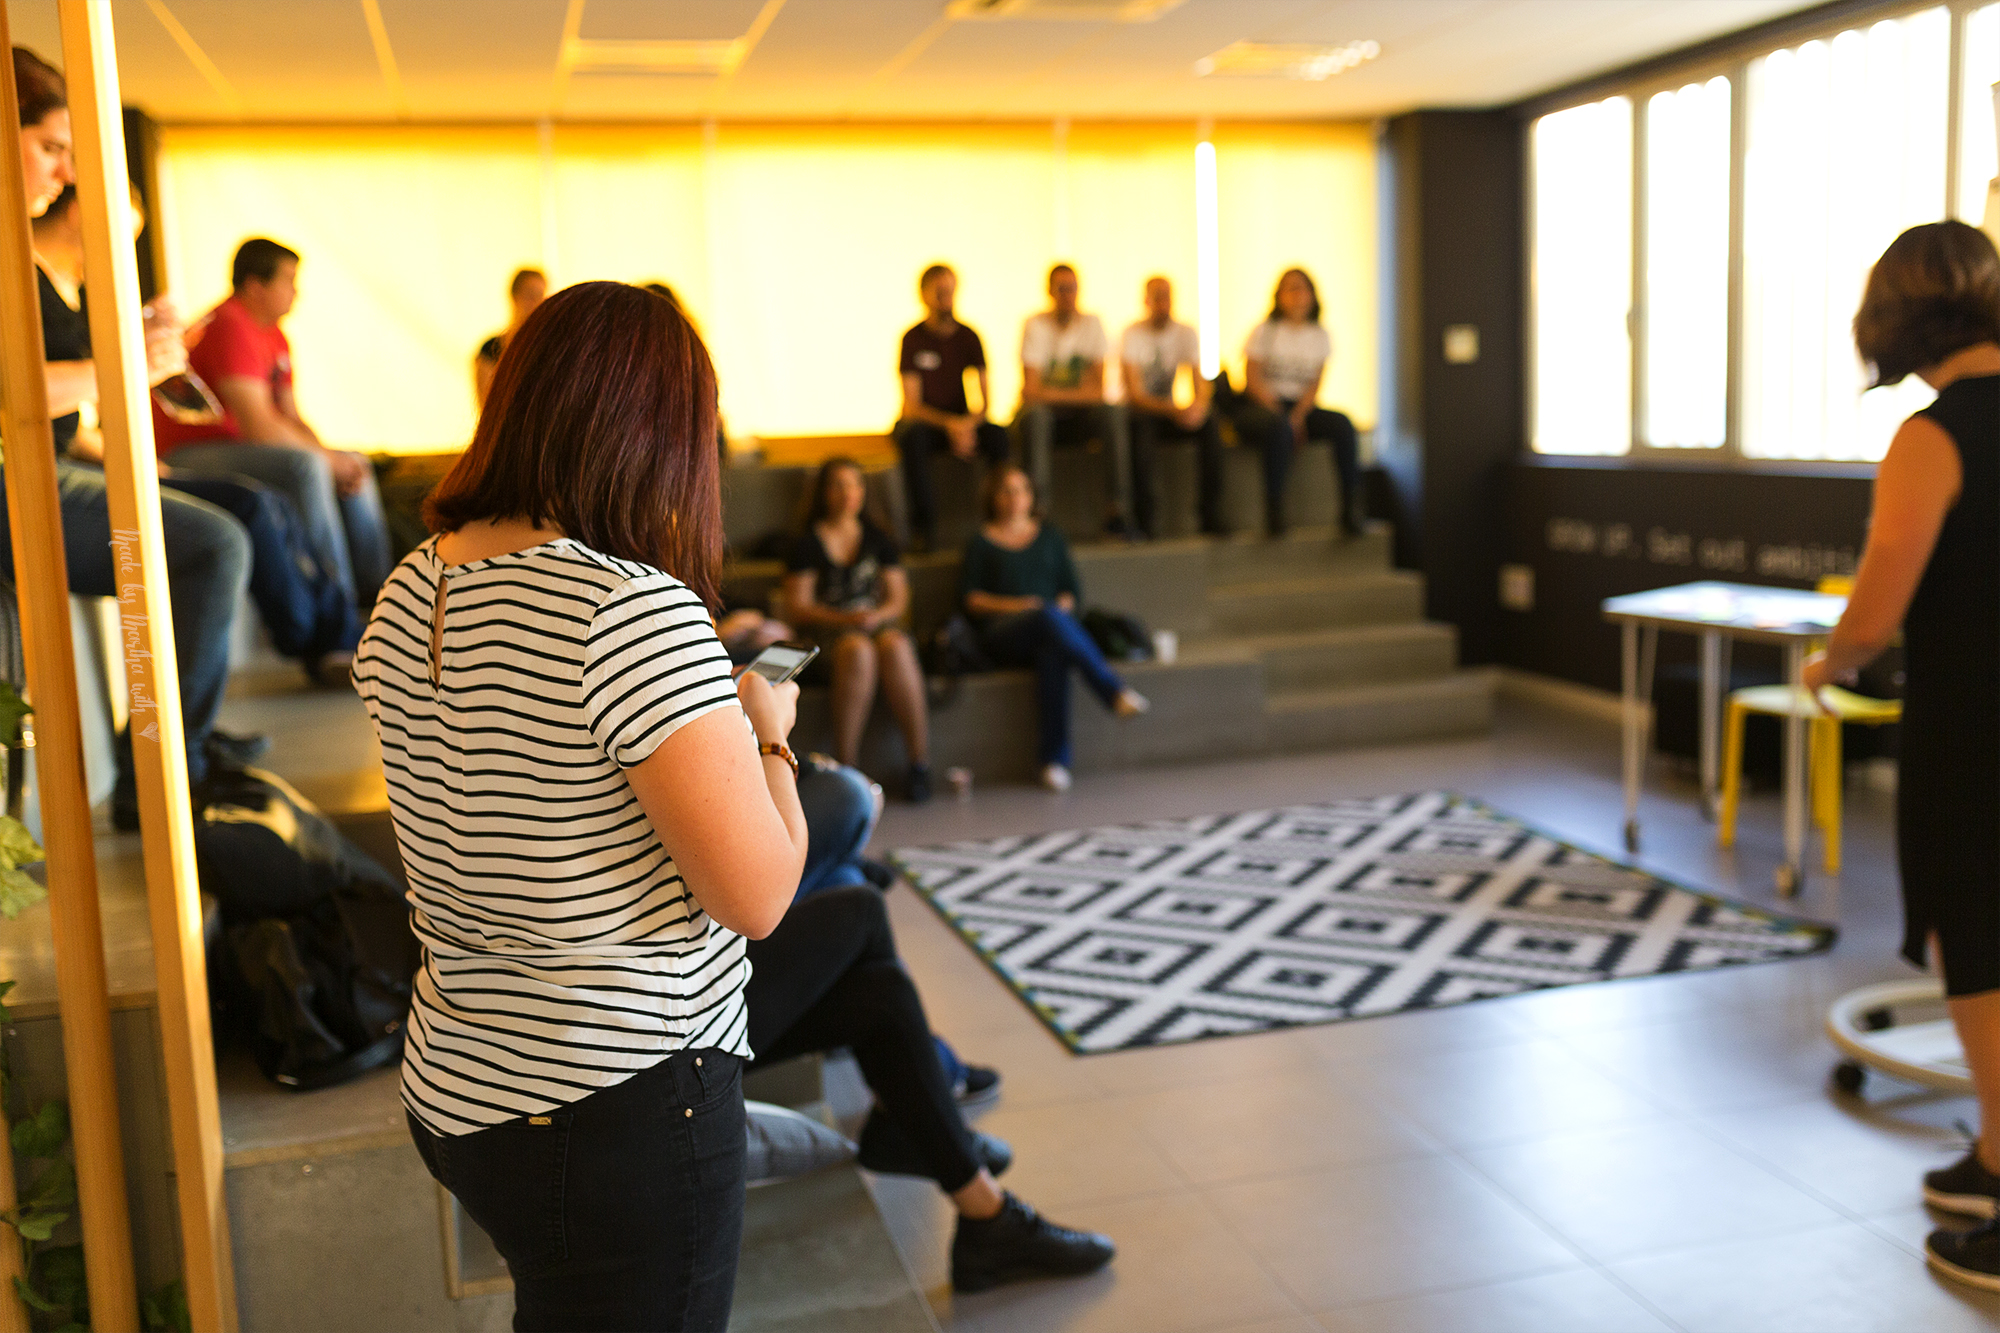
\includegraphics[scale=0.7]{linkuma}
    \caption{Evento de \textit{Yes We Tech} en Link - \textcopyright\ Geek and Tech Girls \cite{linkimage}}}
    \label{linkumaimage}
\end{figure}

\subsection{Usabilidad y UX}
En el campo de la usabilidad y la \textit{User Experience} (UX) se ha dicho mucho con el objetivo de encontrar la clave de un sistema que sea usable y amigable para todos los grupos de usuarios de tecnología que existen actualmente. Se hace necesario para lograr éxito que las interfaces sean sencillas de entender y claras, con una estructura que no haga que el usuario desinstale la aplicación o cierre la pestaña del navegador.\\

Por ello, para este proyecto, en lo que corresponde al trabajo de desarrollo web, he decidido construir mi aplicación web en base a unos principios de diseño actuales y que siguen creciendo con el paso del tiempo.

\subsubsection{Diseño adaptable o \textit{responsive}}
El diseño adaptable establece que un sistema informático (ya sea una página web, un programa de ordenador o una aplicación móvil) debe ser \textbf{reactivo} a la interacción del usuario con el mismo y al entorno en el que se encuentra. Esto quiere decir que ha de ``adaptarse'' a todo tipo de dispositivos donde se esté ejecutando o visualizando. \cite{responsivelink}\\

Ya sea en una pantalla de 24 pulgadas, o un smartphone de 5, el sistema ha de ser capaz de mostrar la misma información y de proporcionar la misma funcionalidad, \textbf{reorganizando los contenidos} de la interfaz para que nada quede inaccesible. En la figura \ref{water} podemos ver de forma gráfica el concepto que aquí se expone.\\

En este sentido, existe un framework de diseño adaptable que nos facilita la tarea de crear un sistema usable en todo tipo de formatos de pantalla, \textbf{Bootstrap} \cite{bootstrap}. Proporciona un conjunto de elementos para el \textit{``layout''} de la aplicación y objetos de interacción como pestañas, botones, paneles, etc.

\begin{figure}
    \centering
    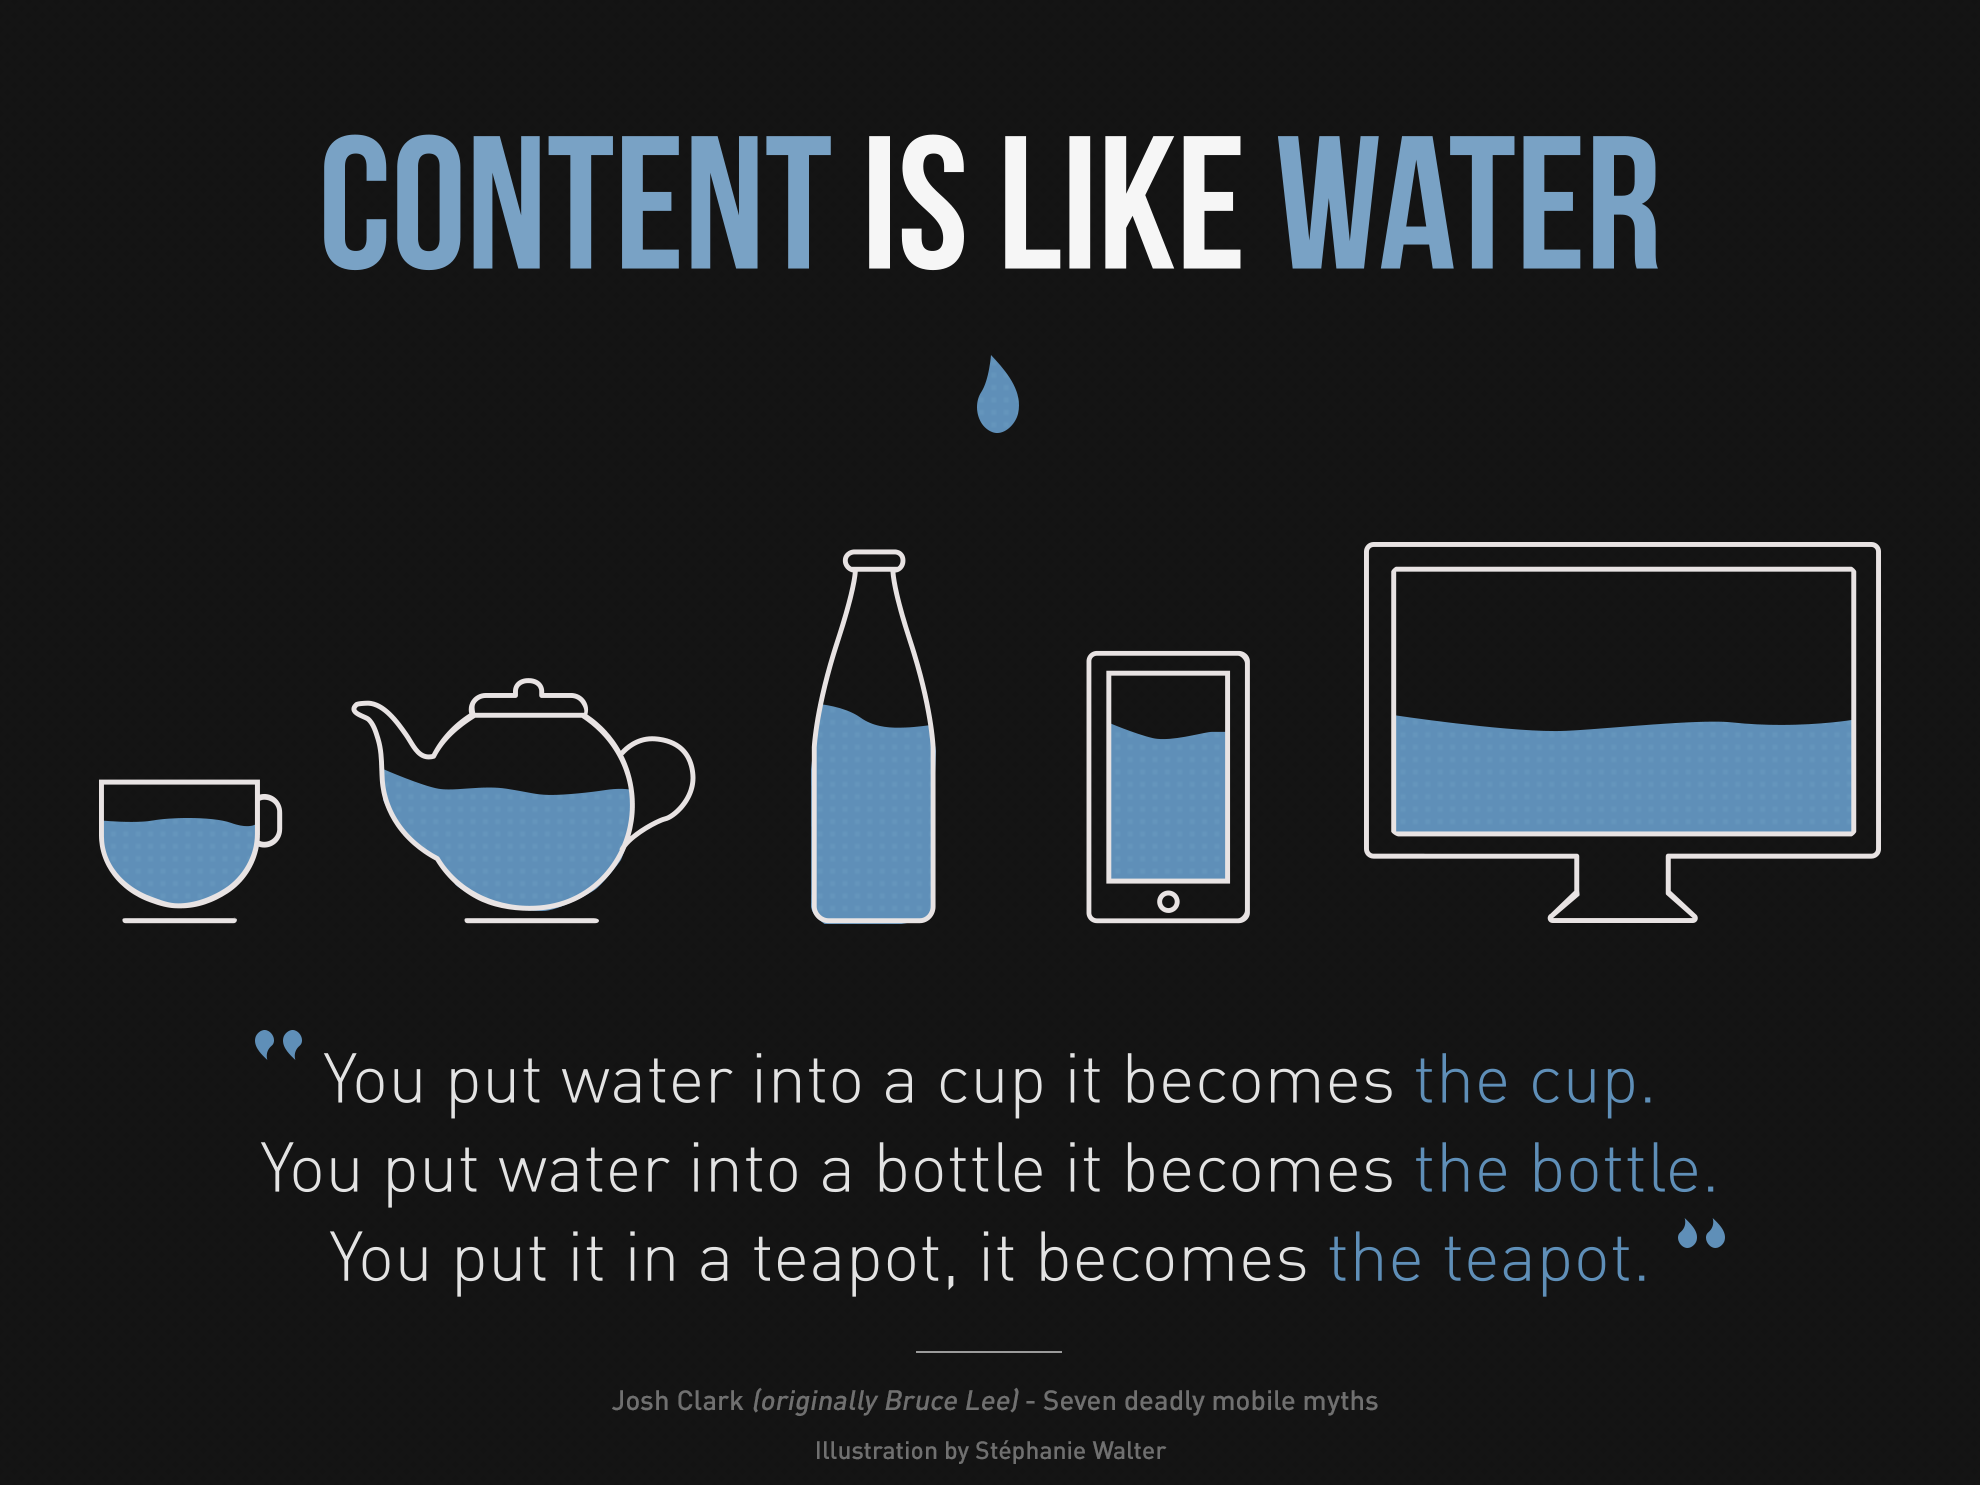
\includegraphics[scale=0.165]{water}
    \caption{\textit{``El contenido es como el agua''} - \textcopyright\ Clark y Walter \cite{contentwater}}
    \label{water}
\end{figure}
